\documentclass[titlepage]{article}
\usepackage{tikz}
\usetikzlibrary{arrows,automata}

\begin{document}
\title{TDT4205 Compiler Technology Problem Set 2}
\maketitle

\section{Problem 1}
\begin{enumerate}[a)]
\item \leavevmodeoo{\vspace{-\baselineskip}}\\
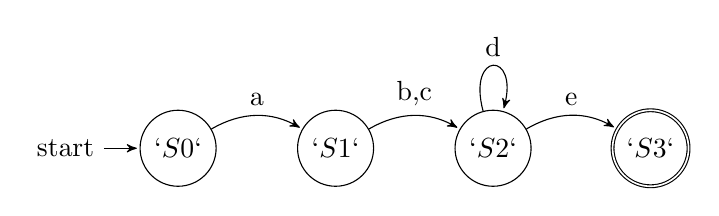
\begin{tikzpicture}[>=stealth',shorten >=1pt,auto,node distance=2cm]
  \node[initial,state]    (S)               {`$S0$`};
  \node[state]            (q1) [right of=S] {`$S1$`};
  \node[state]            (q2) [right of=q1]{`$S2$`};
  \node[state,accepting]  (q3) [right of=q2]{`$S3$`};

  \path[->] (S)  edge [bend left]  node {a}  (q1)
            (q1) edge [bend left]  node {b,c}(q2)
            (q2) edge [bend left]  node {e}  (q3)
                 edge [loop above] node {d}  (q1);
\end{tikzpicture}

\end{enumerate}
\end{document}